\documentclass[doctor,12pt]{styles/iscs-thesis}

%%%%%%%%%%%%%%%%%%%%%%%%%%%%%
% import necessary packages %
%%%%%%%%%%%%%%%%%%%%%%%%%%%%%
\usepackage{newtxtext,newtxmath}      % change font to "Times New Roman"
\usepackage[nottoc]{tocbibind}        % Includes "References" in the table of contents
\usepackage[                          % Add clickable hyper links to references and TOC
  hidelinks,
  dvipdfmx,
  colorlinks = true,
  linkcolor = black,
  urlcolor  = blue,                   % turn URL link to blue color
  citecolor = black,
  anchorcolor = black]{hyperref}
\usepackage[round]{natbib}            % author-year style references, *.bib requires BibTeX format
\usepackage{indentfirst}              % the first paragraph also indent with 2 characters
\usepackage[dvipdfmx]{graphicx}       % zoom the table/figure to the proper size
\usepackage{bmpsize}                  % previous dvipdfm option and this to fix pdf figure error
\usepackage[                          % Bold the Fig. and Table.
  labelfont=bf,
  textfont=md]{caption}
\usepackage{chngpage}
\usepackage[nobiblatex]{xurl}         % long url line breaks
\usepackage{lscape}                   % landscape full page figures
\usepackage{setspace}                 % set page for published paper abstract linespace
\usepackage{ulem}                     % better view for underline
\usepackage{amsmath}                  % package for matrix formular
\usepackage{pifont}                   % package for special symbol

%%%%%%%%%%%%%%%%%%%%%%%%%%%%%
\urlstyle{same}                       % the \url{} links also use Times New Roman font
% \setlength{\parskip}{5pt}           % if you need space before each paragraph, open it

\usepackage{geometry}                 % change the page setting to standard MS Word A4
\geometry{a4paper,left=3.17cm,right=3.17cm,top=2.54cm,bottom=2.54cm}

\setcounter{secnumdepth}{3}           % add the subsubsection into contents
%%%%%%%%%%%%%%%%%%%%%%%%%%%%%

% add Fig. Sx and Table Sx for supplementary section
\newcommand{\appendixsection}{%
  \section{Appendix}% Set supplementary section

  \setcounter{table}{0}% Reset table counter
  \let\oldthetable\thetable% Capture table numbering scheme
  \renewcommand{\thetable}{S\oldthetable}% Prefix table number with S

  \setcounter{figure}{0}% Reset figure counter
  \let\oldthefigure\thefigure% Capture figure numbering scheme
  \renewcommand{\thefigure}{S\oldthefigure}% Prefix figure number with S

  \let\oldchapter\chapter% Copy \chapter into \oldchapter
  \renewcommand{\chapter}{% Update \chapter
    \let\thefigure\oldthefigure% Copy \thefigure into \oldthefigure
    \let\chapter\oldchapter% Restore original \chapter
    \oldchapter% Call original \chapter
  }
}

% 論文の種類とフォントサイズをオプションに
%-------------------
\etitle{Studies on 3D-based Plant Phenotyping by Cross-Scale Sensing}
\jtitle{クロススケールセンシングによる作物の3次元フェノタイピングに関する研究}
%
\eauthor{Haozhou Wang}
\jauthor{王浩舟}
% \jsupervisor{加藤洋一郎  東京大学教授}
\jsupervisor{加藤洋一郎}
\senkou{農学国際専攻(IPADS)}
% \supervisortitle{  郭威   東京大学准教授}
\supervisortitle{東京大学教授}
\date{令和 3 年博士課程入学}
%-------------------
\begin{document}

% \begin{eabstract}
  Abstract abstract abstract, 
\end{eabstract}
\begin{jabstract}
  概要、概要概要概要概要概要概要概要概要概要概要概要概要概要概要概要概要概要
\end{jabstract}

\maketitle

\frontmatter %% 前付け
\tableofcontents % 目次
\listoffigures % 図目次
\listoftables % 表目次
%\lstlistoflistings % ソースコード目次
%-------------------

\mainmatter %% 本文

% \chapter{General Introduction}

\section{Fruits and vegetable production challenges}

% Fruits and vegetables play an important role in human nutrition, as a source of trace elements, vitamins, and minerals. As the \gls{who} suggested for the healthy diet, at least 400 grams of them should be consumed per day to protect against malnutritions (\url{https://www.who.int/news-room/fact-sheets/detail/healthy-diet}). For example, broccoli (\textit{Brassica oleracea} L.) heads, one of the most important components of the global vegetable market, several case studies have demonstrated its great potential to prevent cancer and cardiovascular disease \citep{mahn_overview_2012,latte_health_2011}. However, their supplies and quality can be easily affected by extreme weather events (\url{https://www.bbc.com/news/business-64776969}). Moreover, climate change and global warming also have negative impacts on vegetables, especially lettuce and broccoli which need a cold accumulation period to produce a harvest \citep{bisbis_potential_2018}. In addition, different field management (e.g., tillage, density, and nutrient) also affects the vegetable yield and quality \citep{jackson_onfarm_2004, satodiya_effect_2015}. Hence, to ensure the vegetable supply and quality, it is important to monitor the plants during the growth stages and to take proper management decisions in time.

Fruits and vegetables are important sources of trace elements, vitamins, and minerals in human nutrition. The \gls{who} recommends consuming at least 400 grams of fruits and vegetables per day to prevent malnutrition (\url{https://www.who.int/news-room/fact-sheets/detail/healthy-diet}). For example, broccoli (\textit{Brassica oleracea} L.) heads, which are one of the most important components of the global vegetable market, have shown their great potential to prevent cancer and cardiovascular disease by several case studies \citep{mahn_overview_2012,latte_health_2011}. However, their supply and quality can be easily affected by extreme weather events (\url{https://www.bbc.com/news/business-64776969}). Moreover, climate change and global warming also have negative impacts on vegetables, especially lettuce and broccoli, which need a cold accumulation period to produce a harvest \citep{bisbis_potential_2018}. In addition, different field management practices (e.g., tillage, density, and nutrients) also affect vegetable yield and quality \citep{jackson_onfarm_2004, satodiya_effect_2015}. Hence, it is important to monitor the plants during their growth stages and make proper management decisions promptly to ensure vegetable supply and quality.

% Conventional agriculture management activities, like disease and pest monitoring and selective harvesting, requires heavy manual operations. Such artificial activities pose several challenges. First, judging the disease at the early stage and deciding whether proper harvest often require professional knowledge and can be subject to human errors. 
% Second, the available human labor in agriculture is decreasing nowadays. It is affected by both long-term global events like urbanization and aging population; and short-term pandemics like economic recession and \gls{covid19} \citep{gallardo_adoption_2018,larue_labor_2020}. Such labor shortage raises the labor costs and the costs will be passed on to the consumer end. In this scenario, labor-saving technologies have unprecedented demand. Combined with the fast development of technologies like automation, sensing, big data analysis, computer vision, and artificial intelligence, the agricultural industry has finally gone through the digital agriculture revolution \citep{gallardo_adoption_2018}.

Conventional agricultural management activities for such purposes require significant manual labor and are now facing several challenges. Firstly, they often require professional knowledge and may be subject to human error. Secondly, the availability of human labor in agriculture is currently decreasing due to long-term global events, such as urbanization and aging populations, as well as short-term pandemics, such as economic recessions and \gls{covid19} \citep{gallardo_adoption_2018, larue_labor_2020}. As a result, there is an unprecedented demand for labor-saving technologies. The development of technologies, such as automation, sensing, big data analysis, computer vision, and artificial intelligence, has made it possible to address such demands and thereby spark the digital revolution in the agricultural industry \citep{gallardo_adoption_2018}.

\section{Plant phenotyping techniques}
% background introduction for plant phenotyping
The labor-saving and digitized plant status monitoring, also named plant phenotyping, has been developed and implemented rapidly in recent years \citep{araus_field_2014}. It is defined as ``\textit{the application of methodologies and protocols to measure a specific trait related to plant structure or function with traits ranging from cellular to whole-plant levels}'' \citep{fiorani_future_2013, ghanem_physiological_2015}. Though different workflows are required for different crops and applications, the general workflow of plant phenotyping can be summarized as 1) Data collection, to collect plant or with background data by variate sensors; 2) \gls{roi} extraction, to detect or to segment plant parts at expected levels (e.g. full canopy or single organ) from the collected data; 3) crop traits calculation; and 4) practical or advanced applications.

\subsection{Data collection}
%% platform types -> indoor, outdoor(ground, aerial, satellite)
For the data collection, there are variable sensors for different plant phenotyping purposes. The sensors can be split into environmental sensors (e.g. light intensity, temperature, and humidity) and plant sensors (e.g. organic compounds, plant images) \citep{garlando_plants_2020}. The environmental sensors are often set in a fixed place, as an important component of \gls{iot}, to record environmental factors which are crucial and can affect plant phenotypes \citep{ghanem_physiological_2015}. While plant sensors are often set on and moved with the platforms (Fig.~\ref{fig:int1}). From the indoor (Fig.~\ref{fig:int1}a-d)to the outdoor (Fig.~\ref{fig:int1}e-k), the scale of collected data using these platforms also changes from organ level, individual level to canopy level.

\begin{figure}[htb!]
  \begin{center}
    \resizebox{\textwidth}{!}{
      \includegraphics{figures/int/platforms.pdf}
    }
  \end{center}
  \caption[Example of platforms for plant phenotyping]{
    Example of platforms for plant phenotyping. (a-b) self-designed indoor devices \citep{wu_mvs-pheno_2020,schunck_pheno4d_2021}; (c-d) robotic arms in growth chamber or greenhouse \citep{chaudhury_machine_2018, du_greenhouse_2021}; (e) tractor \citep{kusumam_3d_2017}; (f) ground vehicle \citep{liu_estimation_2017}; (g-h) \gls{ugv} \citep{mcguire_high_2021, qiu_field-based_2019}; (i-j) robotic outdoor instruments \citep{bai_nu-spidercam_2019, jin_exploring_2021}; and (k) \gls{uav} \citep{kierdorf_growliflower_2022}
  }
  \label{fig:int1}
\end{figure}

% From the indoor to the outdoor, the commonly used platforms include self-designed indoor devices \citep{wu_mvs-pheno_2020,schunck_pheno4d_2021}, robotic arms in growth chamber or greenhouse \citep{chaudhury_machine_2018, du_greenhouse_2021}, tractor \citep{kusumam_3d_2017,blok_effect_2021}, ground vehicle \citep{liu_estimation_2017}, \gls{ugv} \citep{mcguire_high_2021,qiu_field-based_2019}, robotic outdoor instruments \citep{bai_nu-spidercam_2019, jin_exploring_2021}, \gls{uav} \citep{kierdorf_growliflower_2022, jang_review_2020}, and even satellite \citep{nguyen_monitoring_2020}. The scale of collected data using these platforms also changes from organ level, individual level to canopy level.


An important part of plant sensors is imaging sensors, which can record the morphological information of crops and are therefore commonly used in many plant phenotyping studies \citep{paulus_measuring_2019, feng_comprehensive_2021}. For example, the infrared, multi- and hyper-spectral imaging sensors were used to calculate several vegetation indices \citep{han_modeling_2019}, like \gls{ndvi}, to assess biomass \citep{jimenez-berni_high_2018}, yield and water stress level \citep{, herrero_yield_2020, romano_use_2011}, and broccoli head freshness \citep{guo_evaluation_2022}. The common \gls{rgb} camera was also used to count plant number \citep{liu_estimating_2022}, plant density \citep{velumani_estimates_2021}, detect the broccoli head \citep{blok_machine_2016}, and access broccoli head quality \citep{stansell_use_2017}. They show the feasibility of imaging sensors in plant phenotyping with great efficiency and non-destructive dependency.

%% 3D sensors
% introduction for 3D phenotyping, method to obtain 3D (passive, active) -> cost limit, choose RGB+SfM
However, these imaging sensors are hard to directly describe the 3D morphological structure of plants, due to occlusion and dimension loss when projecting onto the 2D plane of photosensitive element. As a result, it produces inaccuracies and uncertainties for 3D structure description. With the development of sensing techniques, several studies reviewed the latest available approaches for 3D plant phenotyping \citep{paulus_measuring_2019, okura_3d_2022, kochi_introduction_2021}. Figure~\ref{fig:int2} summarizes some of them which are commonly used, consisting of active and passive sensors.

\begin{figure}[htb!]
  \begin{center}
    \resizebox{\textwidth}{!}{
      \includegraphics{figures/int/recons_sensors.pdf}
    }
  \end{center}
  \caption[Common methods for 3D structure reconstruction]{
    Common methods for 3D structure reconstruction. (a-d) The active sensors rely on projecting lights on the object and analyzing the reflection results, where (d) \acrfull{lidar}; (d2) \acrfull{hls}; (d3) \acrfull{tls}; (d4) \acrfull{als}; (e-f) the passive sensors rely on analyzing the passively received image groups. (e) is a part image of \citep[Fig.~6]{schima_imagine_2016}; (g-h) the \gls{rgb}-based 3D reconstruction algorithms from several perspective images, via (g) conventional geometric deduction and (h) deep learning.
  }
  \label{fig:int2}
\end{figure}

The active sensors use a light source projecting light on the object and analyze the reflection results to obtain the structure. It has two main parts, triangulation and \gls{tof}. The triangulation approach uses the shape changes on the projected straight laser line(s) to obtain the object structure. For example, \citet[Figure~3]{schunck_pheno4d_2021} used a laser line (Fig.~\ref{fig:int2}a) triangulation scanner (Perceptron Scan Works V5, Perceptron Inc., Plymouth, MI, USA) to build a public 3D model database for maize and tomato. The structured light improved the efficiency by projecting an array of lines, often visible or infrared light rather than laser (Fig.~\ref{fig:int2}b). The Microsoft Kinect V1 is a famous \gls{rgbd} camera based on this approach which was released in November 2010. But it was used by a few plant phenotyping studies \citep{nguyen_structured_2015}, since the second version (Kinect V2, released in July 2014) and the third version (Azure Kinect, released in March 2020) with a different \gls{tof} approach and better performance \citep{tolgyessy_evaluation_2021, lachat_assessment_2015} were available. The \acrfull{tof} measures the distance between the sensor and points on the object to obtain its structure. According to the type of light source used, it can be divided into two categories: infrared for \gls{tof} camera (Fig.~\ref{fig:int2}c) and laser for \gls{lidar} (Fig.~\ref{fig:int2}d). Since the sun is a massive source of infrared, infrared-based ToF cameras typically do not perform well in outdoor environments with intense sunlight \citep{tolgyessy_evaluation_2021}; and are therefore commonly used for indoor plant reconstruction applications \citep{martinez_low_2019, zhang_3d_2020, xu_global_2023}. In contrast, the laser is often more tolerant to sunlight due to its stronger energy density, making it widely used in outdoor environments. According to the type of \gls{lidar} sensor, it is consisted of 2D \gls{lidar} scanner \citep{garrido_3d_2015}, 3D \gls{hls} \citep{ma_calculation_2019}, 3D \gls{tls} \citep{wu_accurate_2019, su_estimation_2018, qiu_field-based_2019}, and 3D \gls{als} \citep{ten_biomass_2019, nguyen_uav_2023} for 3D plant phenotyping applications.

The passive sensors rely on analyzing the passively received image groups. The light field camera takes a group of photos with different focal lengths, the shape of object is calculated according to different degrees of clarity caused by the different distances to the sensor (Fig.~\ref{fig:int2}e). 

% Realsense用的Stero Camera没问题,但是Kinect v1是基于红外线的形变,kinectv2是红外线的ToF
% but it seems Kinect V1 uses infrared structured light and Kinect V2 uses the infrared time-of-flight.

% 
% The structure from motion uses the overlapped area among images to estimate the camera poses and object structure. The stereo uses known binocular disparity to obtain structure of object.
% nerf network (learning)

%% software SfM

%% sfm in agricultrual applications.

% \subsection{Data analysis for phenotyping}
% for data analysis.

\subsection{ROI extraction}

\subsubsection{Image analysis}
%% image analysis

%%% traditional CV method

%%% deep learning based method

\subsubsection{3D analysis}
%% 3D data analysis

%%% remove background

%%% segmentation

%%%% individual segmentation

%%%% organ segmentation

\subsection{Traits calculation}
% du_greenhouse_2021 -> 100多个参数

%% 1D 参数

%% 2D 参数

%% 3D 参数

\subsection{Advanced application}

%% 收期预测、光照模拟

\section{Challenges in plant phenotyping}



\section{Objective of this study}

\begin{enumerate}
    \item To develop an almost-automatic 3D reconstruction workflow that can obtain the integrate and high-quality 3D models of destructively sampled broccoli heads.
    \item To develop an unsupervised phenotyping workflow that can automatically segment the broccoli crown part from Objective 1, and calculate several 1D to 3D morphological traits.
    \item To develop an improved workflow for \gls{uav}-based 3D reconstruction broccoli canopy using the 3D to 2D projection and labor-saving deep learning technique, which can obtain better 2D morphological traits of broccoli heads in complex outdoor conditions.
    \item To combine the strengths of the \gls{uav}-based pipeline (high throughput but low quality) and the destructive-based pipeline (high quality but low throughput). Using the auto machine learning regression and the template matching to recover the 3D traits from \gls{uav}-based 2D traits for all broccolis in the field.

\end{enumerate}


\section{Outline of this study}

Chapter 1 is an overview of the study's background information, relative studies, and objectives

Chapter 2 develops and validates the 3D phenotyping pipeline for destructively sampled broccoli heads using the photogrammetry technique, which includes obtaining high-quality plant 3D models and calculating the 3D traits.


Chapter 3 develops and validates the 3D phenotyping pipeline for \gls{uav} sensing on broccoli canopy, includes the 3D to 2D projection pipeline to improve deep-learning-based phenotyping

Chapter 4 tests the idea of cross-scale assimilation of broccoli based on the pipeline built in Chapter 2 and Chapter 3.

Chapter 5 summarizes the general conclusions of this study, and also discusses the research prospects in the future.
\chapter{Workflow for high-throughput data acquisition and 3D reconstruction}

\section{Introduction}

Honbun honbun, honbun honbun \citep{zhao_crop_2019}. 


\section{Methods}


\section{Results}

\section{Discussion}
% \chapter{Workflow for data processing and analyzing}

\section{Introduction}

Honbun honbun, honbun honbun \citep{zhao_crop_2019}. 


\section{Methods}


\section{Results}

\section{Discussion}
% \chapter{Cross indoor and outdoor scale data assimilation}

\section{Introduction}

% what is backward project , what is forward projection

% convert 3D geo-coordinate to 2D pixel coordinate (backward projection); convert 2D pixel coorinate to 3D geo- is not possible, 1) information loss -> using the camera position + roatation + points on the image plane, can only get a ray, rather than a speicify 3D points. reflect to the equation in suppleate (eq.xx) need to solve xxx which is hard. The solution 1. one object from different view, and calculate the intersection points (sfm method), easy to match the polygon for each broccoli, but hard to identify the polygon vertex matches. Plus, different view may have different shapes, can not perfectly match; 2. Find the point at which the ray intersects the surface of the model. difficulties: 对于每一条射线,都要去判断和所有的三角面是否相交,有可能遇到多个相交的三角面(如穿过叶片部分而不是花头)还需要仔细判断到底想交到了哪个面,计算量非常恐怖。一个点需要去和数十万的三角面判断关系,然后一个西兰花头就有几十个点,然后地里面有一万多的西兰花头,使得快速得到结果不太可能。

% 所以在第三章中,使用的规则是,根据grid定点在两个坐标中的位置,直接使用projective transfomration, 进行变换,这样计算比较迅速,而且基于西兰花田地的特点(一个起伏变化不是很大的平地),能大体上保证变换后尺寸比例的正确性,并不影响head traits的计算;但是由于视角等细微的变化,导致位置上的正确性不是很好(Fig.1.1); 为了能更准确的实现可视化,把西兰花头更精准的放回到地里面,需要对这个位置变幻进行进一步的优化

% 另外,由于地里面的尺寸和我们破坏性采样的西兰花,尺寸并不能完美的匹配,因此还需要针对尺寸进行适当的变幻,比较常用的方法是建立一个样地尺寸-db尺寸的线性回归模型,但是由于细小的差距,在我们预实验中,效果并不理想。而选择不同回归模型需要大量的时间去尝试来找到表现最好的,因此采用Auto-ml来节省时间。

the possible solutions 

% challenges:
% 1. ground low quality
% 2. forward to DOM, information loss, unable to find the specific results.
%    -> due to the infomation loss; one possible solution is solve the spot line with meshes (game engine), but very time costy to calculate whether interaction with each vectex,
% 3. model selection -> auto-ml

% note: 西兰花 模型自动选择的必要性

\begin{figure}[htb!]
  \begin{center}
    \resizebox{\textwidth}{!}{
      \includegraphics{figures/xrs/challenges.pdf}
    }
  \end{center}
  \caption[Challenge to forward results from pixel coordinate to geographical coordinate]{
    Challenge to forward results from (a) pixel coordinate on raw image to (b) geographical coordinate on \gls{dom}. The red polygons are broccoli head segmentation results while the blue broken lines are the boundary of the current plot grid. (b) shows the projective transformation on the grid vertices has slight deviations.
  }
  \label{fig:xrs1}
\end{figure}


\section{Methods and Materials}

\begin{figure}[htb!]
  \begin{center}
    \resizebox{\textwidth}{!}{
      \includegraphics{figures/xrs/transform_cp_220331_114_DJI_0289.pdf}
    }
  \end{center}
  \caption[Control points between geographical coordinates on DOM and the pixel coordinate on raw image]{
    Control points between geographical coordinates on DOM and the pixel coordinate on raw image. The blue broken lines are the \gls{roi} boundary of the current grid, the red dots are the control points.
  }
  \label{fig:xrs2}
\end{figure}

Fast Normalized cross-correlation \citet{yoo_fast_2009}


\section{Results}

\begin{figure}[htb!]
  \begin{center}
    \resizebox{\textwidth}{!}{
      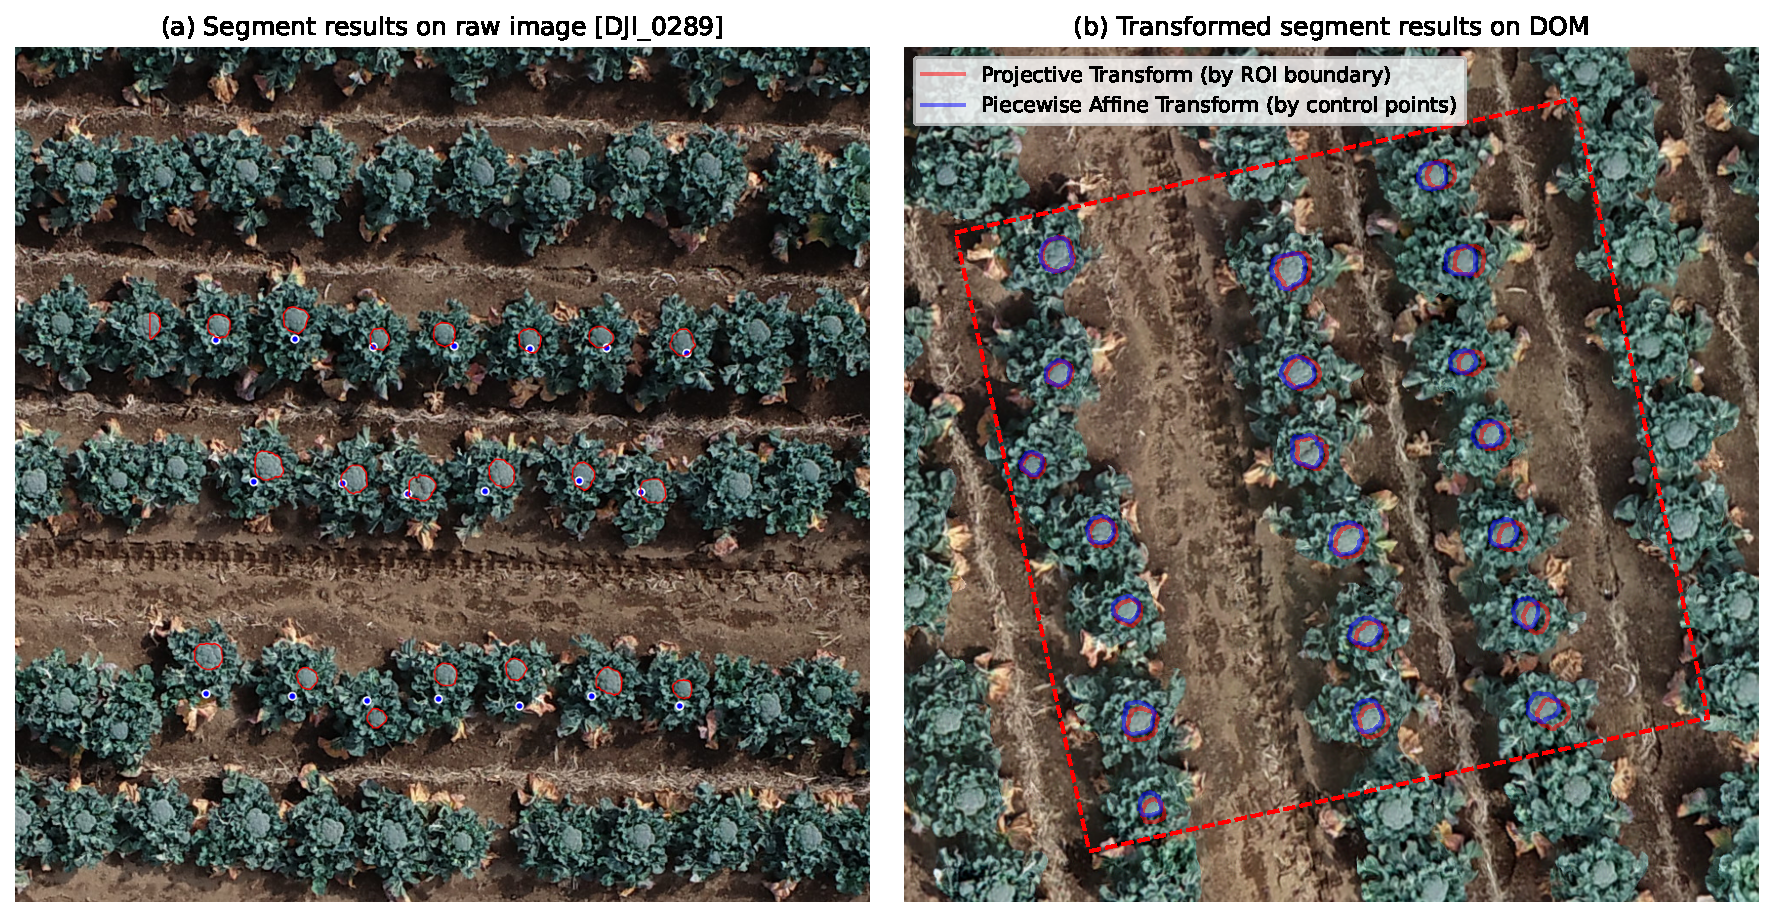
\includegraphics{figures/xrs/trans_compare_220331_114_DJI_0289.pdf}
    }
  \end{center}
  \caption[Head segmentation forward location comparison between projective and piecewise affine transformation]{
    Head segmentation forward location comparison between projective (in Chapter 3) and piecewise affine transformation (this chapter). (a) is the head segmentation results on the raw image. They are forward transformed to corresponding positions on the \gls{dom} using two different transformations.
  }
  \label{fig:xrs3}
\end{figure}

\begin{figure}[htb!]
  \begin{center}
    \resizebox{\textwidth}{!}{
      \includegraphics{figures/xrs/validation4automl.pdf}
    }
  \end{center}
  \caption[Validation for the AutoML calibration model]{
    Validation for the AutoML calibration model.
  }
  \label{fig:xrs4}
\end{figure}

\begin{figure}[htb!]
  \begin{center}
    \resizebox{\textwidth}{!}{
      \includegraphics{figures/xrs/aerial_matched_compare_220405_29.pdf}
    }
  \end{center}
  \caption[The closest matched broccoli head template 3D model]{
    The closest matched broccoli head template 3D model to each aerial segmentation results. Different colors represent different broccoli heads.
  }
  \label{fig:xrs5}
\end{figure}


\section{Discussion}

\section{Conclusion}
% \chapter{General Conclusion}

\section{Overall discussion}

% Virtual plants powered crop data analysis and phenotyping applications.

The plant and its canopy architecture influence the responses and interactions with various environmental factors, which ultimately affects the yield. The conventional analysis methods rely on heavy and repetitive field measured geometry traits along with statistical analysis through whole growing seasons. While the advent of digital twin technology points a very different future, the researchers can operate directly on the virtual plants and preview its impact on the plant immediately verdouw_digital_2021. The fundamental in implementing such technology is to present the 3D crop model (virtual plant) accurately in the computer first, and then implement architecture fine-tuning and phenotyping applications on them. This seminar will summarize recent published papers on how this has been achieved.

Currently, there are three main methods of acquiring virtual plant that can be architecture fine-tuned. 1) By template stitching. chang_3dcap_2022 obtained the database of wheat organ 3D models at different growth stages by destructive sampling and manual measurement of parameters. Then combine those organed to one wheat by random picking and placing with random position angles within the range obtained by real measurements. wen_3d_2021 applied the similar idea for maize. 2) By static deformation. The 3D static model of whole maize (in point cloud format) was obtained by 3D reconstruction. The maize model was then automatically segmented to organs, and these segmented parts were transformed by applying geometric transformations to implement changes in architecture liu_canopy_2021. 3) By parametric approximation. The L-system was used to construct a parameter adjustable virtual crop model and then adjusted the parameters to approximate the real crop by three-view photos cieslak_l-system_2021. This process was also reflected in the implementation of CG modelling. For example, the general shape of the plant was obtained through relatively simple geometries, and then photo-quality texture mapping was used to obtain a very realistic CG model mikami_hidden_2022.

Several phenotyping applications can be simulated on the adjustable virtual 3D plant models. 1) The ray-tracing technologies can be applied to simulate lights within the canopy. For example, analysis of the contributions of foliar and nonfoliar tissues chang_3dcap_2022, leaf inclination angles liu_canopy_2021, and row spacing he_modeling_2021 to canopy photosynthesis efficiency of each crop. 2) The LiDAR point cloud simulation technology can be used to simulate point clouds from the virtual canopy. For the canopy traits which are easy to get from virtual plants but hard from the real field, the corresponding models between features from simulated point cloud and traits from virtual canopy can be trained, and then applied on the field scanned LiDAR data to inverse the actual data liu_estimating_2017. 3) the CG rendering techniques can decrease the workload of data annotating in the phenotyping data processing by deep learning. The rending engine can yield CG photos that are very close to the real world. At the same time, by adjusting the model texture to solid pure color, the corresponding labelled information for both CG photos mikami_hidden_2022 and point clouds chaudhury_3d_2020 can be generated in batch from random virtual canopies.



\section{Future work}


%-------------------
\bibliographystyle{plainnat} % 参考文献
\bibliography{styles/bibtex} %
%-------------------

% % Add Acknowladgement to TOC
\chapter*{Acknowledgements}
\addcontentsline{toc}{chapter}{Acknowledgements}

I would like to express my sincere gratitude to my thesis supervisor, Prof. Yoichiro Kato of the Graduate School of Agricultural and Life Sciences, for his invaluable advice, support, guidance, and encouragement throughout my doctoral research journey. He has constantly challenged and guided me to push the boundaries of my research and finally bring me to the point of accomplishing my degree.

I would also like to extend my thanks to the members of my thesis committee, [todo] committee memeber's names, for their valuable feedback and insights. Their contributions have significantly improved the quality and relevance of my research.

Furthermore, I would like to thank Dr. Wei Guo. He not only served almost like a role of an advisor who greatly helped with my doctoral studies but also as a close friend who gave me many valuable suggestions for both academic and daily life in Japan. Also thank Dr. Yuji Yamasaki from The University of Tokyo, Dr. Yuya Fukano from Chiba University, Dr. Wenli Zhang from Beijing University of Technology, Dr. Yun Shi and Dr. Yulin Duan from Chinese Academy of Agricultural, and Dr. Feng Wang from Chinese Academy of Forestry, for providing me with advanced resources and excellent academic support.

I would also like to thank Naomi Morinaga, Kozue Wada, Alexander Feldman, Kunihiro Kodama, Masanori Ishii, and all the technical support staffs of \gls{isas} for providing me with a conducive research environment and excellent support for fieldwork and document-related work. It enabled me to freely explore and develop my research interests.

I am also extremely grateful to my labmates. Tang Li is a good friend who helped me a lot with deep learning and life in Japan, and Nishida Erika contributed greatly to the broccoli fieldwork. I also thank my tutors, Thum Chun Hau and Jaesuk IM, for their kind help, and all my other friends for being the pillars of my life.

I would also like to express my gratitude to my family for their constant support, encouragement, and love, especially my girlfriend who has never appeared in my actual life and has allowed me to fully focus on my academic work.

Thank you all for being an integral part of my doctor journey and for helping me achieve this milestone.
% \section*{Journals}

\noindent
Related to the doctor studies

\begin{enumerate}
  \item Zhang, W., Peng, X., Cui, G., \textbf{Wang, H.}, Takata, D., Guo, W., 2023. Tree Branch Skeleton Extraction from Drone-Based Photogrammetric Point Cloud. \textit{Drones} 7, 65. \url{https://doi.org/10.3390/drones7020065}
  \item Drofova, I., Guo, W., \textbf{Wang, H.}, Adamek, M., 2023. Use of scanning devices for object 3D reconstruction by photogrammetry and visualization in virtual reality. \textit{Bulletin of Electrical Engineering and Informatics} 12, 868–881. \url{https://doi.org/10.11591/eei.v12i2.4584}
  \item Zhao, L., Guo, W., Wang, J., \textbf{Wang, H.}, Duan, Y., Wang, C., Wu, W., Shi, Y., 2021. An Efficient Method for Estimating Wheat Heading Dates Using UAV Images. \textit{Remote Sensing} 13, 3067. \url{https://doi.org/10.3390/rs13163067}
  % \item \textbf{Wang, H.}, Yang, T.-R., Waldy, J., Kershaw, J.A., 2021b. Estimating Individual Tree Heights DBHs from Vertically Displaced Spherical Image Pairs. \textit{Mathematical and Computational Forestry \& Natural-Resource Sciences} 13, 1–14. \url{https://mcfns.net/index.php/Journal/article/view/13.1}
  \item \textbf{Wang, H.}, Duan, Y., Shi, Y., Kato, Y., Ninomiya, S., Guo, W., 2021a. EasyIDP: A python package for intermediate data processing in UAV-based plant phenotyping. \textit{Remote Sensing} 13, 2622. \url{https://doi.org/10.3390/rs13132622}
  % \item Hsu, Y.-H., Kershaw, J.A., Ducey, M.J., Yang, T.-R., \textbf{Wang, H.}, 2021. Sampling with probability proportional to prediction (3P sampling) using covariates derived from spherical images. \textit{Canadian Journal of Forest Research} 51, 1140–1147. \url{https://doi.org/10.1139/cjfr-2020-0498}
  \item Feldman, A., \textbf{Wang, H}., Fukano, Y., Kato, Y., Ninomiya, S., Guo, W., 2021. EasyDCP: An affordable, high-throughput tool to measure plant phenotypic traits in 3D. \textit{Methods in Ecology and Evolution} 12, 1679–1686. \url{https://doi.org/10.1111/2041-210X.13645}
  % \item Dai, X., Ducey, M.J., Kershaw, J.A., \textbf{Wang, H.}, 2021a. Sector subsampling for basal area ratio estimation: an alternative to big BAF sampling. \textit{Canadian Journal of Forest Research} 1–9. \url{https://doi.org/10.1139/cjfr-2020-0496}
  % \item Dai, X., Ducey, M.J., \textbf{Wang, H.}, Yang, T.-R., Hsu, Y.-H., Ogilvie, J., Kershaw, J.A., Jr, 2021b. Biomass estimates derived from sector subsampling of 360° spherical images. \textit{Forestry: An International Journal of Forest Research} 94, 565–575. \url{https://doi.org/10.1093/forestry/cpab023}
  % \item \textbf{Wang, H.}, Kershaw, J.A., Yang, T.-R., Hsu, Y.-H., Ma, X., Chen, Y., 2020. An Integrated System for Estimating Forest Basal Area from Spherical Images. \textit{Mathematical and Computational Forestry \& Natural-Resource Sciences} 12, 0–14. \url{http://mcfns.net/index.php/Journal/article/view/12.1}
  % \item \textbf{Wang, H.}, Han, D., Mu, Y., Jiang, L., Yao, X., Bai, Y., Lu, Q., Wang, F., 2019. Landscape-level vegetation classification and fractional woody and herbaceous vegetation cover estimation over the dryland ecosystems by unmanned aerial vehicle platform. \textit{Agricultural and Forest Meteorology} 278, 107665. \url{https://doi.org/10.1016/j.agrformet.2019.107665}
\end{enumerate}

\noindent
Not related to the doctor studies

\begin{enumerate}
  \item \textbf{Wang, H.}, Yang, T.-R., Waldy, J., Kershaw, J.A., 2021b. Estimating Individual Tree Heights DBHs from Vertically Displaced Spherical Image Pairs. \textit{Mathematical and Computational Forestry \& Natural-Resource Sciences} 13, 1–14. \url{https://mcfns.net/index.php/Journal/article/view/13.1}
  \item Hsu, Y.-H., Kershaw, J.A., Ducey, M.J., Yang, T.-R., \textbf{Wang, H.}, 2021. Sampling with probability proportional to prediction (3P sampling) using covariates derived from spherical images. \textit{Canadian Journal of Forest Research} 51, 1140–1147. \url{https://doi.org/10.1139/cjfr-2020-0498}
  \item Dai, X., Ducey, M.J., Kershaw, J.A., \textbf{Wang, H.}, 2021a. Sector subsampling for basal area ratio estimation: an alternative to big BAF sampling. \textit{Canadian Journal of Forest Research} 1–9. \url{https://doi.org/10.1139/cjfr-2020-0496}
  \item Dai, X., Ducey, M.J., \textbf{Wang, H.}, Yang, T.-R., Hsu, Y.-H., Ogilvie, J., Kershaw, J.A., Jr, 2021b. Biomass estimates derived from sector subsampling of 360° spherical images. \textit{Forestry: An International Journal of Forest Research} 94, 565–575. \url{https://doi.org/10.1093/forestry/cpab023}
  \item \textbf{Wang, H.}, Kershaw, J.A., Yang, T.-R., Hsu, Y.-H., Ma, X., Chen, Y., 2020. An Integrated System for Estimating Forest Basal Area from Spherical Images. \textit{Mathematical and Computational Forestry \& Natural-Resource Sciences} 12, 0–14. \url{http://mcfns.net/index.php/Journal/article/view/12.1}
  \item \textbf{Wang, H.}, Han, D., Mu, Y., Jiang, L., Yao, X., Bai, Y., Lu, Q., Wang, F., 2019. Landscape-level vegetation classification and fractional woody and herbaceous vegetation cover estimation over the dryland ecosystems by unmanned aerial vehicle platform. \textit{Agricultural and Forest Meteorology} 278, 107665. \url{https://doi.org/10.1016/j.agrformet.2019.107665}
\end{enumerate}

\section*{Conferences}

\noindent
Related to the doctor studies

\begin{enumerate}
  \item \textbf{Wang, H.}, Tang, L., Nishida, E., Fukano, Y., Kato, Y., Guo, W. Sept 27-30, 2022. Estimate Optimal Harvest Time by Cross-scale Assimilated Digital Broccoli Farmland (\textbf{poster}), \textit{7th International Plant Phenotyping Symposium: "Plant Phenotyping for a Sustainable Future"}, Wageningen, Netherlands.
  \item \textbf{Wang, H.}, Kato, Y., Guo, W. May 21-22, 2022. Procedural Geometric Modeling for Plant Phenomics by Blender: Case Study of Maize (\textbf{oral}), \textit{農業情報学会JSAI 2022年次大会}, Kyoto, Japan.
  \item \textbf{Wang, H.}, Tang, L., Nishida, E., Fukano, Y., Kato, Y., Guo, W. July 20-22, 2021. Cost-efficient broccoli head phenotyping using aerial imagery and SfM-based weakly supervised learning (\textbf{poster}), \textit{The 8th International Horticulture Research Conference}, Nanjing, Jiangsu, China.
  \item \textbf{Wang, H.}, Kato, Y., Guo, W., June 3-4, 2021. EasyIDP: A python package for intermediate data processing in UAV based plant phenotyping (\textbf{poster}), \textit{超分野植物科学研究会の第1回研究集会 2021}, Zoom online, Tokyo, Japan.
  \item \textbf{Wang, H.}, Kato, Y., Guo, W., May 22, 2021. EasyIDP: A python package for intermediate data processing in UAV based plant phenotyping (\textbf{poster}), \textit{農業情報学会JSAI 2021年次大会}, Zoom online, Tokyo, Japan.
  \item Feldman, A., \textbf{Wang, H.}, Fukano, Y., Kato, Y., Ninomiya, S., Guo, W., February 24-27, 2020. Affordable high-throughput processing of handheld camera images of container plants to phenotypic data (\textbf{poster}), \textit{Phenome 2020}, Tucson Convention Center, Tucson, Arizona, U.S.
  \item Feldman, A., \textbf{Wang, H.}, Fukano, Y., Guo, W., October 22-25, 2019. Affordable high-throughput processing of multi-scale images to phenotypic data (\textbf{poster}). \textit{The 6th International Plant Phenotyping Symposium}, Nanjing, Jiangsu, China.
\end{enumerate}

\noindent
Not related to the doctor studies

\begin{enumerate}
  \item \textbf{Wang, H.}, Kershaw, J.A., June 23-25, 2019. Estimating Forest Attributes from Spherical Images (\textbf{oral}, \textbf{poster}). \textit{The Western Mensurationists 2019 Annual Meeting}, Kamloops Hotel and Conf. Center, Kamloops, British Columbia, Canada.
  \item \textbf{Wang, H.},, Kershaw, J.A., March 23, 2018. Measuring Plant Area Index (PAI) from panorama photo images (\textbf{oral}). \textit{The 25th Annual UNB Graduate Research Conference (GRC)}, Wu Conference Center, Fredericton, New Brunswick, Canada.
  \item \textbf{Wang, H.}, Kershaw, J.A., November 5-7, 2017. Extracting DBH Measurements from RGB Photo Images (\textbf{oral}). \textit{The Northeastern Mensurationists 2017 Annual Meeting}, The Inn at Saratoga. Saratoga Springs, New York, U.S.
  \item \textbf{Wang, H.}, Wang, F., Yao, X., Mu, Y., Bai, Y., Lu, Q., August 20-25, 2017 . UAV-HiRAP: A novel method to improve landscape-level vegetation classification and coverage fraction estimation with unmanned aerial vehicle platform (\textbf{oral}). \textit{The 12th International Congress of Ecological (INTECOL)}, China National Convention Center, Beijing, China.
\end{enumerate}

\section*{Source Code}

\noindent
Easy-Series Software packages

\begin{enumerate}
  \item EastAMS - A GUI plugin tool for Agisoft Metashape with extended functions for smart agriculture. \url{https://github.com/UTokyo-FieldPhenomics-Lab/EasyAMS}
  \item EastBPY - The wrapper for blender python API without pip install extra packages. \url{https://github.com/UTokyo-FieldPhenomics-Lab/EasyBPY}
  \item EasyIDP - A handy tool for dealing with region of interest (ROI) on the image reconstruction (Metashape \& Pix4D) outputs, mainly in agriculture applications. \url{https://github.com/UTokyo-FieldPhenomics-Lab/EasyIDP}
  \item  EasyDCP - Easy Dense Cloud Phenotyping. \url{https://github.com/UTokyo-FieldPhenomics-Lab/EasyDCP}
\end{enumerate}

\noindent
Projects

\begin{enumerate}
  \item UAVbroccoli - Protocol for broccoli data analysis by Metashape. \url{https://github.com/UTokyo-FieldPhenomics-Lab/UAVbroccoli}
  \item Foldio360\_3D\_Reconstruct\_Platform - a protocol for easy indooor 3D reconstruction for small objects. \url{https://github.com/UTokyo-FieldPhenomics-Lab/Foldio360_3D_Reconstruct_Platform}
\end{enumerate}

\noindent
Website maintainer

\begin{enumerate}
  \item \url{www.global-wheat.com} - The website for global wheat dataset. \url{https://github.com/UTokyo-FieldPhenomics-Lab/global-wheat.github.io}
  \item \url{2023.mlcas.site} - The website for Fifth International Workshop on Machine Learning for Cyber-Agricultural Systems (MLCAS2023). \url{https://github.com/UTokyo-FieldPhenomics-Lab/mlcas2023.github.io}
  \item \url{lab.fieldphenomics.com} - The official website for Laboratory of Field Phenomics at UTokyo. \url{https://github.com/UTokyo-FieldPhenomics-Lab/utokyo-fieldphenomics-lab.github.io}
  \item \url{mlcas2021.github.io} - The website for Third International Workshop on Machine Learning for Cyber-Agricultural Systems (MLCAS2021). \url{https://github.com/mlcas2021/mlcas2021.github.io}
\end{enumerate}

\end{document}